% \iffalse
\let\negmedspace\undefined
\let\negthickspace\undefined
\documentclass[journal,12pt,twocolumn]{IEEEtran}
\usepackage{cite}
\usepackage{amsmath,amssymb,amsfonts,amsthm}
\usepackage{algorithmic}
\usepackage{graphicx}
\usepackage{textcomp}
\usepackage{xcolor}
\usepackage{txfonts}
\usepackage{listings}
\usepackage{enumitem}
\usepackage{mathtools}
\usepackage{gensymb}
\usepackage{comment}
\usepackage[breaklinks=true]{hyperref}
\usepackage{tkz-euclide}
\usepackage{listings}
\usepackage{gvv}
\def\inputGnumericTable{}
\usepackage[latin1]{inputenc}
\usepackage{color}
\usepackage{array}
\usepackage{longtable}
\usepackage{calc}
\usepackage{multirow}
\usepackage{hhline}
\usepackage{ifthen}
\usepackage{lscape}

\newtheorem{theorem}{Theorem}[section]
\newtheorem{problem}{Problem}
\newtheorem{proposition}{Proposition}[section]
\newtheorem{lemma}{Lemma}[section]
\newtheorem{corollary}[theorem]{Corollary}
\newtheorem{example}{Example}[section]
\newtheorem{definition}[problem]{Definition}
\newcommand{\BEQA}{\begin{eqnarray}}
\newcommand{\EEQA}{\end{eqnarray}}
\newcommand{\define}{\stackrel{\triangle}{=}}
\theoremstyle{remark}
\newtheorem{rem}{Remark}
\begin{document}

\bibliographystyle{IEEEtran}
\vspace{3cm}

\title{NCERT Discrete - 10.5.2.19}
\author{EE23BTECH11007 - Aneesh Kadiyala$^{*}$% <-this % stops a space
}
\maketitle
\newpage
\bigskip

\renewcommand{\thefigure}{\theenumi}
\renewcommand{\thetable}{\theenumi}
%fi

\vspace{3cm}
\textbf{Question 10.5.2.19:} Subba Rao started work in 1995 at an annual salary of Rs. 5000 and received an increment of Rs. 200 each year. In which year did his income reach Rs. 7000?
\\
\solution
\begin{enumerate}
\item
Let Subba Rao's initial salary $a_0$ = Rs. 5000
\\
Let Subba Rao's increment $d$ = Rs. 200
\\
Subba Rao's salary after n years = $a_n$ = $a_0 + (n - 1)d$
\\
\[7000 = 5000 + (n - 1)(200)\]
\[2000 = (n - 1)(200)\]
\[n = 11\]

$\implies$Subba Rao's income reaches Rs. 7000 eleven years after he started working.

Therefore, Subba Rao's income reached Rs. 7000 in the year 2006.

\item \textbf{Finding $x(n)$}

The series is an arithmetic progression.
\[x(n) = x(0) + nd\]
where $d$ is the common difference.

It is given that initial value $x(0)$ is 5000 and common difference $d$ is 200.
\[\implies x(n) = (5000 + 200n)(u(n))\]
as $x(n) = 0 \forall n < 0$.

\begin{figure}[h!]
    \centering
    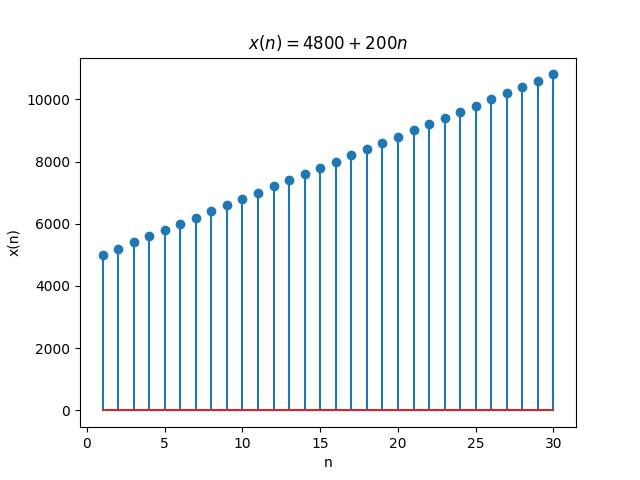
\includegraphics[width=\columnwidth]{figs/10_5_2_19.png}
\end{figure}

\item \textbf{Z-transform of $x(n)$}

Let Z-transform of $x(n)$ be $X(z)$. Let U(z) be the Z-transform of $u(n)$.

\[X(z) = \sum_{n = -\infty}^{\infty} (5000 + 200n)(u(n))(z^{-n})\]
\[X(z) = 5000\sum_{n = -\infty}^{\infty} u(n)(z^{-n}) + 200\sum_{n = -\infty}^{\infty}n(u(n))(z^{-n})\]
Using differentiation in Z-domain property,\\Z-transform of $nx(n) = -z\frac{d}{dz}X(z)$
\[\implies X(z) = 5000U(z) + 200(-z)\frac{d}{dz} U(z)\]
\[X(z) = \frac{5000}{1 - z^{-1}} + 200(-z)(-\frac{1}{z^2(1-z^{^-1})^2})\]
\[X(z) = 5000(1 - z^{-1})^{-1} + 200\frac{z}{(z - 1)^2}\]
\[X(z) = 5000z(z - 1)^{-1} + 200z(z - 1)^{-2}\]

Region of Convergence (ROC) of $z$ is $|z| > 1$.

\end{enumerate}
\end{document}